\documentclass[12pt,letterpaper]{article}
\usepackage{fullpage}
\usepackage[top=2cm, bottom=4.5cm, left=2.5cm, right=2.5cm]{geometry}
\usepackage{amsmath,amsthm,amsfonts,amssymb,amscd}
\usepackage{lastpage}
\usepackage{enumerate}
\usepackage{fancyhdr}
\usepackage{mathrsfs}
\usepackage{xcolor}
\usepackage{graphicx}
\usepackage{hyperref}
\usepackage{tikz}
\usepackage{enumitem}

\hypersetup{%
  colorlinks=true,
  linkcolor=blue,
  linkbordercolor={0 0 1}
}

\setlength{\parindent}{0.0in}
\setlength{\parskip}{0.05in}

% Edit these as appropriate
\newcommand\course{}
\newcommand\hwnumber{4}                  % <-- homework number
\newcommand\NetIDa{Ivan Zhytkevych}
% \newcommand\NetIDb{Ivan Zhytkevych}

\pagestyle{fancyplain}
\headheight 35pt
\lhead{\NetIDa}
% \lhead{\NetIDa\\\NetIDb}                 % <-- Comment this line out for problem sets (make sure you are person #1)
\chead{\textbf{\Large Homework \hwnumber (Part 1)}}
\rhead{\course \\ \today}
\lfoot{}
\cfoot{}
\rfoot{\small\thepage}
\headsep 1.5em


\def\set{\@ifstar{\@set}{\@set*}}


\begin{document}


\section*{Problem 4.26}

\begin{center}
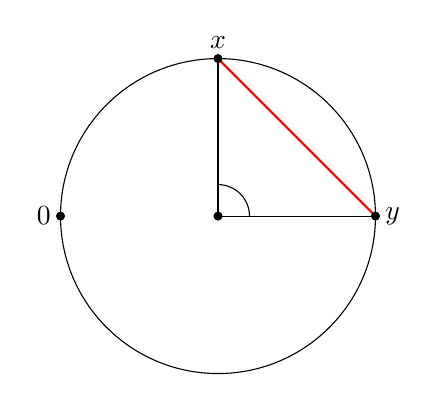
\begin{tikzpicture}[scale=2]
    \node [left] at (-1, 0) {$0$};
    \draw[fill] (-1, 0) circle [radius=0.025];
    \node [left] at (0, 0) {};
    \draw[fill] (0, 0) circle [radius=0.025];

    \draw (0, 0) circle [radius=1];
    \draw (0, 0) -- (0,1);
    \draw (1, 0) -- (0, 0);
    \draw[red, thick] (1, 0) -- (0, 1);

    \draw (0, 0.2) arc [radius=0.2, start angle=90, end angle=0];

    \node [above] at (0, 1) {$x$};
    \draw[fill] (0, 1) circle [radius=0.025];
    \node [right] at (1, 0) {$y$};
    \draw[fill] (1, 0) circle [radius=0.025];

\end{tikzpicture}
\end{center}

\[ \Omega = \{(x, y) : x, y \in (0, 2\pi)\} \]

\begin{center}
    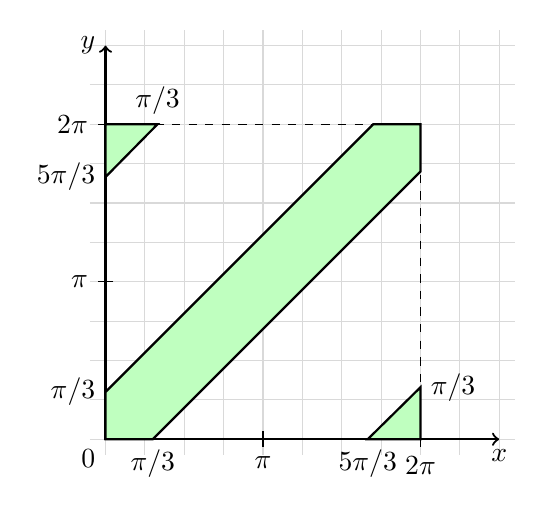
\begin{tikzpicture}
        \draw[step=0.5, gray!30, thin, xshift=0cm, yshift=0cm] (-0.2, -0.2) grid (5.2,5.2);
        \draw[thick, <->] (0, 5) node[left]{$y$}
            -- (0, 0) node[below left]{$0$}
            -- (5, 0) node[below]{$x$};

        \draw (2, .1) -- (2, -.1) node[below]{$\pi$};
        \draw (4, .1) -- (4, -.1) node[below]{$2\pi$};
        \draw (.1, 2) -- (-.1, 2) node[left]{$\pi$};
        \draw (.1, 4) -- (-.1, 4) node[left]{$2\pi$};
       
        \draw[dashed] (0, 4) -| (4, 0);

        \draw[fill=green!25, thick] (0.6, 0) node[below]{$\pi/3$} -- (4, 3.4) -- (4, 4)
            -- (3.4, 4)-- (0, 0.6) node[left]{$\pi/3$}
            -- (0, 0) -- cycle;

        \draw[fill=green!25, thick] (3.33, 0) node[below]{$5\pi/3$}
            -- (4, 0.66) node[right]{$\pi/3$} -- (4, 0) -- cycle;
        \draw[fill=green!25, thick] (0, 3.33) node[left]{$5\pi/3$}
            -- (0.66, 4) node[above]{$\pi/3$} -- (0, 4) -- cycle;

    \end{tikzpicture}
\end{center}

\[ A = \{ (x, y) \in \Omega : |x-y| < \frac{\pi}{3}
    \text{ or } (2\pi - y) + x < \frac{\pi}{3} 
    \text{ or } (2\pi -x) + y < \frac{\pi}{3} \} \]

    \begin{gather*}
        \left[
        \begin{array}{ll}
            \begin{cases}
                x - y < \frac{\pi}{3} \\
                y - x < \frac{\pi}{3} \\
            \end{cases} \\
            2\pi - y + x < \frac{\pi}{3} \\
            2\pi - x + y < \frac{\pi}{3}
        \end{array}
        \right.
    \end{gather*}

    \[ \mu(A) = 4\pi^2 -
        \left(\frac{\pi}{3}\right)^2
        + \left(\frac{\pi}{3}\right)^2 = 
        4\pi^2 - \frac{25}{9}\pi^2 + \frac{1}{9}\pi^2 =
        \frac{4}{3}\pi^2
    \]

    \[ P(A) = \frac{1}{3} \]

%%%%%%%%%%%%%%%%%%%%%%%%%%%%%%%%%%%%%%%%%%%%%%%%%%%%%%%%%%%%%%%%%%%%%%%%%%%%%%%

    \section*{Problem 4.27}


\begin{center}
    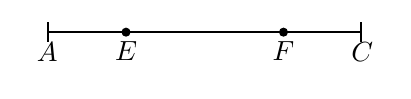
\begin{tikzpicture}
        \draw[|-|, thick] (0, 0) node[below]{$A$} -- (4,0) node[below]{$C$};
        \draw[fill] (1, 0) circle [radius=0.05] node[below]{$E$};
        \draw[fill] (3, 0) circle [radius=0.05] node[below]{$F$};
    \end{tikzpicture}

    \[ \Omega = \left\{ (e,f) : e, f \in (0, \sqrt{13}) \right\} \]
    \[ A = \left\{ (e,f) : \frac{ e^2 }{ (\sqrt{13} - f)^2 } \geq 3 \right\} \]
    \[ f \geq -\frac{1}{\sqrt{3}} e + \sqrt{13} \]

    \[ e = \sqrt{13}: f = \sqrt{13} - \frac{\sqrt{13}}{\sqrt{3}} = \sqrt{13}\left( 1 -
    \frac{1}{\sqrt{3}} \right) \]

    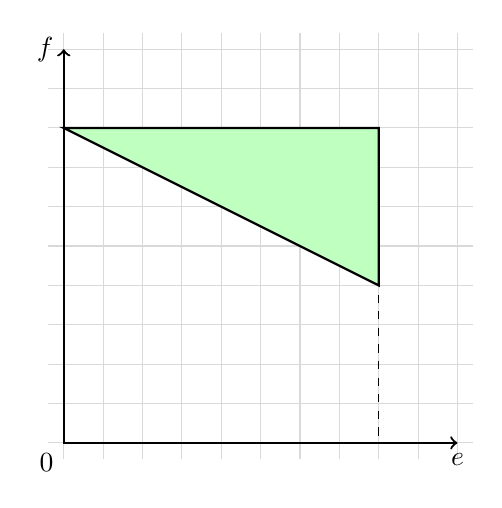
\begin{tikzpicture}
        \draw[step=0.5, gray!30, thin, xshift=0cm, yshift=0cm] (-0.2, -0.2) grid (5.2,5.2);
        \draw[thick, <->] (0, 5) node[left]{$f$}
            -- (0, 0) node[below left]{$0$}
            -- (5, 0) node[below]{$e$};

        \draw[dashed] (0, 4) -| (4, 0);

        \draw[fill=green!25, thick] (0, 4) -- (4, 2) -- (4, 4)
            -- (3.4, 4) -- cycle;

    \end{tikzpicture}

    \[ \mu(A) = \frac{1}{2} \left( \sqrt{13} \cdot (\sqrt{13} - \sqrt{13}(1 - \frac{1}{\sqrt{3}}))
    \right) = \frac{13}{2}\left( 1 - 1 + \frac{1}{\sqrt{3}} \right) = \frac{13}{2\sqrt{3}} \]
    \[ \mu(\Omega) = 13 \]
    \[ P(A) = \frac{1}{2\sqrt{3}} \]
\end{center}

%%%%%%%%%%%%%%%%%%%%%%%%%%%%%%%%%%%%%%%%%%%%%%%%%%%%%%%%%%%%%%%%%%%%%%%%%%%%%%%%%%%%%

\newpage

Further assume the $\Omega$ is set using the following declaration:
\[ \Omega = \{ (\varepsilon_1, \dots, \varepsilon_j) : \varepsilon_i = \pm 1, \sum \varepsilon_i = k \} \]
Where $k$ is $y$ coordinate of destination point and $j$ is $x$ coordinate of one.
\section*{Problem 4.28}

\begin{enumerate}[label=(\alph*)]

    \item \begin{itemize}
        
        \item [(1)] \[ (0, 0) \rightarrow (2n, 0) \]
            \[ S_1 > 0, \dots, S_{2n-1} > 0 \]
            \begin{gather*}
                L_{(1, 1)}^{+} (2n -1, 1) = L_{(1, 1)}(2n-1,1) - L_{(1,-1)}(2n-1,1) = \\
                = L_{(0, 0)}(2n-2, 0) - L_{(0, 0)}(2n-2,2) =
                C_{2n-2}^{n-1} - C_{2n-2}^{n} = \\
                = \frac{(2n-2)!}{(n-1)! (n-1)!} - \frac{(2n-2)!}{n! (n-2)!} =
                (2n-2)! \left( \frac{1}{((n-1)!)^2} - \frac{1}{n!(n-2)!}  \right) = \\
                = \frac{(2n-2)!}{(n-1)!} \left( \frac{1}{(n-1)!} - \frac{n-1}{n!} \right) =
                \frac{(2n-2)!}{(n-1)!} \left( \frac{n-n+1}{n!} \right) =
                \frac{(2n-2)!}{(n-1)!n!}
            \end{gather*}

        \item [(2)] \[ (0, 0) \rightarrow (2n, 0) \]
            \[ S_1 \geq 0, \dots, S_{2n-1} \geq 0 \]
            \begin{gather*}
                L_{(1,1)}^{\geq 0} (2n, 0) = L_{(1,1)}(2n,0) - L_{(1, -3)} (2n, 0) =
                L_{(0,0)} (2n-1, -1) - L_{(0, 0)} (2n-1,3) = \\
                C_{2n-1}^{n} - C_{2n-1}^{n-2} =
                (2n-1)! \left( \frac{1}{n! (n-1)!} - \frac{1}{(n-2)!(n+1)!}\right) = \\
                = (2n-1)! \frac{n+1-n+1}{(n+1)! (n-1)!} = \frac{2(2n-1)!}{(n+1)! (n-1)!}
            \end{gather*}

    \end{itemize}


\end{enumerate}


\end{document}

